\documentclass[12pt,letterpaper, onecolumn]{exam}
\usepackage[lmargin=71pt, tmargin=1.2in]{geometry}  %For centering solution box
\lhead{STAT 479\\}
\rhead{HW 5\\}
\thispagestyle{empty}   %For removing header/footer from page 1
\usepackage{amsmath}
\usepackage{amssymb}
\usepackage{graphicx}
\usepackage{hyperref}
\usepackage{booktabs}
\setlength{\parindent}{0pt}
\setlength{\parskip}{1em}
\setlength{\topsep}{0pt}
\setlength{\partopsep}{0pt}
\usepackage{enumitem}
\usepackage{titlesec}
\usepackage{tikz-cd}
\titlespacing{\section}{0pt}{*0.2}{*0.2}

\usetikzlibrary{bayesnet}

\newcommand{\DKL}[2]{D_{\textrm{KL}}\left[#1 \;\|\; #2\right]}
\newcommand{\sbr}[1]{\left[#1\right]}
\newcommand{\rbr}[1]{\left(#1\right)}
\DeclareMathOperator{\E}{\mathbb{E}}
\DeclareMathOperator*{\argmin}{\mathrm{arg\,min}}
\DeclareMathOperator*{\argmax}{\mathrm{arg\,max}}

\usepackage{makecell}
\usepackage{arydshln}
\usepackage{bm}


\usepackage{tikz}
\newcommand*\circled[1]{
\tikz[baseline=(char.base)]{\node[shape=circle,draw,inner sep=1pt] (char) {#1};}
}
 
% xun
\newcommand{\Gcal}{\mathcal{G}}
\newcommand{\Ical}{\mathcal{I}}
\newcommand{\Hcal}{\mathcal{H}}
\newcommand{\Ucal}{\mathcal{U}}
\newcommand{\Tcal}{\mathcal{T}}
\newcommand{\Ncal}{\mathcal{N}}
\newcommand{\Cbs}{\boldsymbol{C}}
\newcommand{\Sbs}{\boldsymbol{S}}
\newcommand{\Pa}{\text{Pa}}
\newcommand{\De}{\text{De}}
\newcommand{\Nd}{\text{Nd}}
            


\begin{document}

\begingroup
    \centering
    \LARGE STAT 479: Homework 5\\[0.5em]
    \large Due: 11:59PM Mar 18, 2025 by Canvas\\[0.5em]
\endgroup
\rule{\textwidth}{0.4pt}
\pointsdroppedatright   %Self-explanatory
\printanswers
\renewcommand{\solutiontitle}{\noindent\textbf{Answer:}\enspace}

\vspace{-20pt}
\begin{questions}
\vspace{-10pt}

\question[20 points] \textbf{True-False Conceptual Questions}\droppoints

Write TRUE or FALSE for each of these statements.

\begin{parts}
    \part The Bayesian Information Criterion (BIC) includes a penalty term for model complexity, discouraging overly complex models even if they fit the data well.
    \part The Chow-Liu algorithm can learn Bayesian networks with arbitrary structure, including cycles.
    \part In a causal graphical model, observing a common effect (collider) of two variables can create a spurious association between them, even if they were originally independent.
    \part In causal discovery, controlling for a confounder ensures that any observed association between two variables must be causal.
    \part The Expectation-Maximization (EM) algorithm improves the model parameters at each iteration by directly maximizing the likelihood of the observed data.
    \part The likelihood function computed during EM is guaranteed to increase or remain constant at each iteration.
    \part Variational inference approximates the posterior distribution by converting inference into an optimization problem that minimizes the Kullback-Leibler (KL) divergence.
    \part The Evidence Lower Bound (ELBO) is a key objective in variational inference, providing a tractable lower bound on the log-likelihood.
    \part The mean-field approximation in variational inference assumes that latent variables are independent, simplifying computation but potentially reducing accuracy.
    \part Unlike Markov Chain Monte Carlo (MCMC), variational inference always produces an unbiased estimate of the posterior.
\end{parts}

\begin{solution}
    \begin{parts}
        \part
        \part
        \part
        \part
        \part
        \part
        \part
        \part
        \part
        \part
    \end{parts}
\end{solution}


\question[20 points] \textbf{Deriving EM Updates for a Gaussian Mixture Model (GMM)}\droppoints

A Gaussian Mixture Model assumes that data points are generated from a mixture of \( K \) Gaussian distributions, each with a mean \( \mu_k \), covariance \( \Sigma_k \), and a mixing weight \( \pi_k \). As introduced in class, the Expectation-Maximization (EM) algorithm iteratively estimates these parameters.

\begin{parts}
    \part \textbf{Setting Up the Model}
    
    We model the data as being drawn from \( K \) Gaussian components:
    \[
    p(x | \theta) = \sum_{k=1}^{K} \pi_k \mathcal{N}(x | \mu_k, \Sigma_k)
    \]
    where \( \pi_k \) are the mixing weights summing to 1, and \( \mathcal{N}(x | \mu_k, \Sigma_k) \) is a Gaussian density function.
    Which of the following best describes the latent variables in the GMM framework?
    \begin{choices}
        \choice The mixing weights \( \pi_k \) that determine the prior probability of each Gaussian component.
        \choice The covariance matrices \( \Sigma_k \), which control the shape of each Gaussian distribution.
        \choice The component assignments \( z_n \), which indicate which Gaussian component generated each data point.
        \choice The observed data points \( x_n \), which follow a mixture of Gaussians.
    \end{choices}
    \part \textbf{Expectation Step (E-Step)}

    In the E-step, we compute the posterior responsibility \( \gamma_{nk} \), which represents the probability that data point \( x_n \) was generated by component \( k \):

    \[
    \gamma_{nk} = p(z_n = k | x_n, \theta^{(t)}) = \frac{\pi_k^{(t)} \mathcal{N}(x_n | \mu_k^{(t)}, \Sigma_k^{(t)})}{\sum_{j=1}^{K} \pi_j^{(t)} \mathcal{N}(x_n | \mu_j^{(t)}, \Sigma_j^{(t)})}
    \]

    What is the main role of \( \gamma_{nk} \) in the EM algorithm?

    \begin{choices}
        \choice It represents the maximum likelihood estimate of the Gaussian parameters.
        \choice It updates the mixing weights to reflect the proportion of data points assigned to each cluster.
        \choice It acts as a "soft" assignment of each data point to the Gaussian components.
        \choice It maximizes the log-likelihood function directly.
    \end{choices}

    \part \textbf{Maximization Step (M-Step)}

    In the M-step, we update the parameters of the Gaussians by maximizing the expected complete-data log-likelihood. The updates are:

    \[
    \pi_k^{(t+1)} = \frac{1}{N} \sum_{n=1}^{N} \gamma_{nk}
    \]

    \[
    \mu_k^{(t+1)} = \frac{\sum_{n=1}^{N} \gamma_{nk} x_n}{\sum_{n=1}^{N} \gamma_{nk}}
    \]

    \[
    \Sigma_k^{(t+1)} = \frac{\sum_{n=1}^{N} \gamma_{nk} (x_n - \mu_k^{(t+1)})(x_n - \mu_k^{(t+1)})^T}{\sum_{n=1}^{N} \gamma_{nk}}
    \]
    What does the M-step accomplish?
    \begin{choices}
        \choice It reassigns each data point to a single Gaussian component.
        \choice It updates the model parameters to maximize the likelihood given the current soft assignments.
        \choice It computes the posterior probability of each data point belonging to a Gaussian component.
        \choice It eliminates one Gaussian component per iteration to simplify the model.
    \end{choices}
    
    \part \textbf{Convergence and Likelihood Maximization}

    The EM algorithm repeats the E-step and M-step iteratively until convergence, typically when the log-likelihood:

    \[
    \log p(X | \theta) = \sum_{n=1}^{N} \log \sum_{k=1}^{K} \pi_k \mathcal{N}(x_n | \mu_k, \Sigma_k)
    \]

    stabilizes.

    Which of the following statements is \textbf{true} regarding the convergence properties of EM?

    \begin{choices}
        \choice EM always finds the global maximum of the likelihood function.
        \choice EM maximizes a lower bound on the likelihood at each iteration, ensuring non-decreasing likelihood.
        \choice EM can decrease the likelihood in some iterations.
        \choice EM requires computing second-order derivatives to estimate parameter updates.
    \end{choices}
    
\end{parts}

\begin{solution}
    \begin{parts}
        \part
        \part
        \part
        \part
    \end{parts}
\end{solution}


\question[20 points] \textbf{Causal Discovery}\droppoints


Causal discovery aims to infer causal relationships from observational data, often using DAGs to represent causality. Consider the following DAG:

\[
X \rightarrow Z \leftarrow Y, \quad X \rightarrow W \rightarrow Y
\]

Answer the following questions about this causal structure.

\begin{parts}
    \part Based on d-separation, are \(X\) and \(Y\) independent given no observed variables?
    \part Suppose we condition on \(Z\). Are \(X\) and \(Y\) independent then?
    \part If you want to estimate the causal effect of \(X\) on \(Y\), should you adjust for \(W\)? Why or why not?
    \part Suppose an additional variable \(U\) is added, where \(U \rightarrow X\) and \(U \rightarrow Y\). Explain how \(U\) acts as a confounder and how you would adjust for it to estimate the causal effect of \(X\) on \(Y\).
\end{parts}

\begin{solution}
    \begin{parts}
        \part
        \part
        \part
        \part
    \end{parts}
\end{solution}


\clearpage
\question[20 points] \textbf{I-Equivalence and Structure Discovery}\droppoints

Consider a Bayesian network structure learning problem where we aim to discover the best graphical representation of a given dataset. The \textbf{I-equivalence class} of a Bayesian network refers to the set of all graph structures that encode the same set of conditional independence relationships.

\begin{parts}
    \part \textbf{Defining I-Equivalence:} Two Bayesian networks are I-equivalent if they represent the same conditional independence relationships. Given the following two structures, determine whether they are I-equivalent and explain why.
    \[
    G_1: A \rightarrow B \rightarrow C, \quad G_2: A \leftarrow B \rightarrow C
    \]
    \part \textbf{Learning DAGs vs. Learning I-Equivalence Classes:} Explain why learning the true DAG structure from observational data is harder than learning its I-equivalence class. What additional information would we need to uniquely determine the true DAG?

    \part \textbf{Graph Reversibility in I-Equivalence:} Suppose we have two DAGs that belong to the same I-equivalence class. How can we determine whether we can reverse an edge direction in one DAG while still preserving the same conditional independence structure? Provide an example.

    \part \textbf{Implications for Causal Discovery:} If two Bayesian networks are I-equivalent, does that mean they imply the same causal relationships? Why or why not?
\end{parts}

\begin{solution}
    \begin{parts}
        \part
        \part
        \part
        \part
    \end{parts}
\end{solution}

\question[20 points]\textbf{Understanding Lower Bounds in Probabilistic Models}\droppoints

When training probabilistic models, we often approximate the data likelihood using a lower bound because directly computing the likelihood is intractable. We can define a sequence of progressively tighter bounds as follows:

\[
\mathcal{L}_k(\mathbf{x}) = \mathbb{E}_{\mathbf{z}^{(1)}, \dots, \mathbf{z}^{(k)} \sim q_{\mathbf{\phi}}(\mathbf{z} \mid \mathbf{x})} \left[ \log \frac{1}{k} \sum_{i=1}^k \frac{p_{\mathbf{\theta}}(\mathbf{x}, \mathbf{z}^{(i)})}{q_{\mathbf{\phi}}(\mathbf{z}^{(i)} \mid \mathbf{x})} \right].
\]

\begin{parts}
    \part \textbf{Jensen’s Inequality Refresher:} Jensen’s inequality states that for a concave function \( f(x) \),
    \[
    f( \mathbb{E}[X] ) \geq \mathbb{E}[ f(X) ].
    \]
    Show how Jensen’s inequality implies that
    \[
    \log p(\mathbf{x}) \geq \mathcal{L}_k(\mathbf{x})
    \]
    for any $k \in \mathbb{N}$. Remember, $\log(\cdot)$ is a concave function.
    \part \textbf{Why More Samples Help:} Show that \( \mathcal{L}_k(\mathbf{x}) \) gets tighter as \( k \) increases: \(\mathcal{L}_{k+1}(\mathbf{x}) > \mathcal{L}_k(\mathbf{x}) \).

    You can use the following lemma without proof:
    
    \emph{Lemma}: Let $I_k \subset [k+1] := \{1, \ldots, k+1\}$ with $|I_k| = k$ be a uniformly distributed subset of distinct indices from $[k+1]$. Then for any sequence of numbers $a_1, \ldots, a_{k+1}$,
    \begin{equation}\label{eq:new-bound-lemma}
    \mathbb{E}_{I_k} \sbr{ \frac{\sum_{i \in I_k} a_i}{ k} }
    = { \sum_{i=1}^{k+1} a_i \over k+1}
    \end{equation}
\end{parts}

The above two results show that
\[
\log p(\mathbf{x})
\geq \mathcal{L}_{k+1}(\mathbf{x})
\geq \mathcal{L}_{k}(\mathbf{x}).
\]
However, the above inequalities do not guarantee $\mathcal{L}_k(\mathbf{x}) \rightarrow \log p(\mathbf{x})$ when $k \rightarrow \infty$. (The proof is left as an exercise to the reader. Or you can come to my office hours.)

\begin{solution}
    \begin{parts}
        \part
        \part
    \end{parts}
\end{solution}

\clearpage


\question[0 points] \textbf{OPTIONAL Markov Chain Monte Carlo Programming}\droppoints

\textbf{This question is an OPTIONAL programming exercise. It will not impact your grade.}

Nowadays, statistical modeling of sport data has become an important part of sports analytics and is often a critical reference for the managers in their decision-making process. In this part, we will work on a real world example in professional sports. Specifically, we are going to use the data from the 2013-2014 Premier League, the top-flight English professional league for men’s football clubs, and build a predictive model on the number of goals scored in a single game by the two opponents. Bayesian hierarchical model is a good candidate for this kind of modeling task. We model each team’s strength (both attacking and defending) as latent variables. Then in each game, the goals scored by the home team is a random variable conditioned on the attacking strength of the home team and the defending strength of the away team. Similarly, the goals scored by the away team is a random variable conditioned on the attack strength of the away team and the defense strength of the home team. Therefore, the distribution of the scoreline of a specific game is dependent on the relative strength between the home team A and the away team B, which also depends on the relative strength between those teams with their other opponents.

\newcolumntype{K}[1]{>{\centering\arraybackslash}p{#1}}

{\fontsize{8}{10}\selectfont
\begin{table*}[h!] %[!htbp]
\caption{2013-2014 Premier League Teams}
\vspace{2mm}
\setlength\tabcolsep{0.7pt}
\begin{tabular}{|c || *{1}{K{3cm}} | *{1}{K{3cm}} | *{1}{K{3cm}} | *{1}{K{3cm}} | *{1}{K{3cm}} |}
\hline
Index & 0 & 1 & 2 & 3 & 4 \\
Team & Arsenal & Aston Villa & Cardiff City & Chelsea & Crystal Palace \\
\hline
\hline
Index & 5 & 6 & 7 & 8 & 9 \\
Team & Everton & Fulham & Hull City & Liverpool & Manchester City \\
\hline
\hline
Index & 10 & 11 & 12 & 13 & 14 \\
Team & Manchester United & Newcastle United & Norwich City & Southampton & Stoke City \\
\hline
\hline
Index & 15 & 16 & 17 & 18 & 19 \\
Team & Sunderland & Swansea City & Tottenham Hotspurs & West Bromwich Albion & West Ham United \\
\hline
\end{tabular}
\label{teams}
\end{table*}
}

Here we consider using the same model as described by \href{https://www.tandfonline.com/doi/full/10.1080/02664760802684177}{Baio and Blangiardo (2010)}. The Premier League has 20 teams, and we index them as in Table~\ref{teams}. Each team would play 38 matches every season (playing each of the other 19 teams home and away), which totals 380 games in the entire season. For the $g$-th game, assume that the index of home team is $h(g)$ and the index of the away team is $a(g)$.
The observed number of goals $ (y_{g0}, y_{g1}) $ of home and away team is modeled as independent Poisson random variables:
\begin{equation}
y_{gj} | \theta_{gj} \sim \textrm{Poisson}(\theta_{gj}), \quad j = 0,1
\end{equation}
where $\theta = (\theta_{g0},\theta_{g1})$ represents the scoring intensity in the $g$-th game for the team playing at home $(j = 0)$ and away $(j = 1)$, respectively. We put a log-linear model for the $\theta$s:
\begin{equation}
\log \theta_{g0} = home + att_{h(g)} - def_{a(g)}
\end{equation}
\begin{equation}
\log \theta_{g1} = att_{a(g)} - def_{h(g)}
\end{equation}
Note that team strength is broken into attacking and defending strength. And home represents home-team advantage, and in this model is assumed to be constant across teams. The prior on the home is a normal distribution:
\begin{equation}
home \sim \mathcal{N} (0, \tau_0^{-1})
\end{equation}
where we set the precision $\tau_0 = 0.0001$.

The team-specific attacking and defending effects are modeled as:
\begin{equation}
att_t \sim \mathcal{N} (\mu_{att}, \tau_{att}^{-1})
\end{equation}
\begin{equation}
def_t \sim \mathcal{N} (\mu_{def}, \tau_{def}^{-1})
\end{equation}
We use conjugate priors as the hyper-priors on the attack and defense means and precisions:
\begin{equation}
\mu_{att} \sim \mathcal{N} (0, \tau_{1}^{-1})
\end{equation}
\begin{equation}
\mu_{def} \sim \mathcal{N} (0, \tau_{1}^{-1})
\end{equation}
\begin{equation}
\tau_{att} \sim \textrm{Gamma} (\alpha,\beta)
\end{equation}
\begin{equation}
\tau_{def} \sim \textrm{Gamma} (\alpha,\beta)
\end{equation}
where the precision $\tau_1 = 0.0001$, and we set parameters $\alpha = \beta = 0.1$.

This hierarchical Bayesian model can be represented using a directed acyclic graph as shown in Figure~\ref{dag}.

\begin{figure}[ht]
\centering
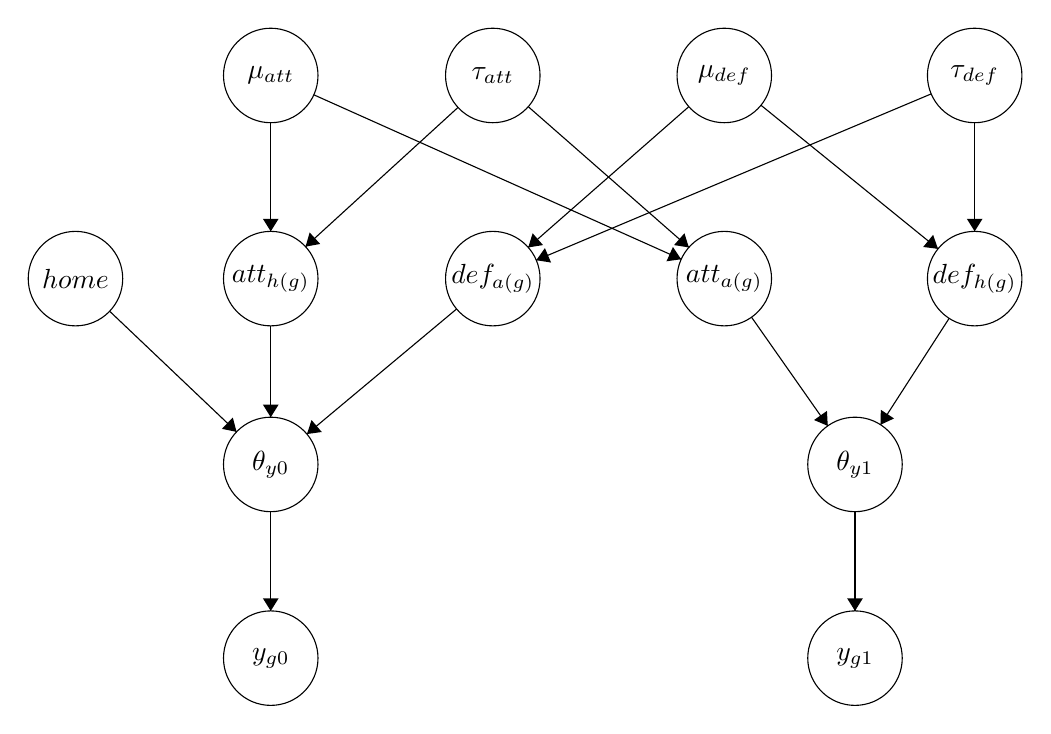
\begin{tikzpicture}[scale=0.2]
\tikzstyle{every node}+=[inner sep=0pt]
\draw [black] (25.1,-42.3) circle (3);
\draw (25.1,-42.3) node {$y_{g0}$};
\draw [black] (62.2,-42.3) circle (3);
\draw (62.2,-42.3) node {$y_{g1}$};
\draw [black] (25.1,-30) circle (3);
\draw (25.1,-30) node {$\theta_{y0}$};
\draw [black] (62.2,-30) circle (3);
\draw (62.2,-30) node {$\theta_{y1}$};
\draw [black] (53.9,-18.2) circle (3);
\draw (53.9,-18.2) node {$att_{a(g)}$};
\draw [black] (69.8,-18.2) circle (3);
\draw (69.8,-18.2) node {$def_{h(g)}$};
\draw [black] (12.7,-18.2) circle (3);
\draw (12.7,-18.2) node {$home$};
\draw [black] (25.1,-18.2) circle (3);
\draw (25.1,-18.2) node {$att_{h(g)}$};
\draw [black] (39.2,-18.2) circle (3);
\draw (39.2,-18.2) node {$def_{a(g)}$};
\draw [black] (39.2,-5.3) circle (3);
\draw (39.2,-5.3) node {$\tau_{att}$};
\draw [black] (25.1,-5.3) circle (3);
\draw (25.1,-5.3) node {$\mu_{att}$};
\draw [black] (53.9,-5.3) circle (3);
\draw (53.9,-5.3) node {$\mu_{def}$};
\draw [black] (69.8,-5.3) circle (3);
\draw (69.8,-5.3) node {$\tau_{def}$};
\draw [black] (25.1,-33) -- (25.1,-39.3);
\fill [black] (25.1,-39.3) -- (25.6,-38.5) -- (24.6,-38.5);
\draw [black] (62.2,-33) -- (62.2,-39.3);
\fill [black] (62.2,-39.3) -- (62.7,-38.5) -- (61.7,-38.5);
\draw [black] (68.18,-20.72) -- (63.82,-27.48);
\fill [black] (63.82,-27.48) -- (64.68,-27.08) -- (63.84,-26.53);
\draw [black] (55.63,-20.65) -- (60.47,-27.55);
\fill [black] (60.47,-27.55) -- (60.42,-26.6) -- (59.6,-27.18);
\draw [black] (69.8,-8.3) -- (69.8,-15.2);
\fill [black] (69.8,-15.2) -- (70.3,-14.4) -- (69.3,-14.4);
\draw [black] (67.04,-6.47) -- (41.96,-17.03);
\fill [black] (41.96,-17.03) -- (42.9,-17.18) -- (42.51,-16.26);
\draw [black] (51.65,-7.28) -- (41.45,-16.22);
\fill [black] (41.45,-16.22) -- (42.39,-16.07) -- (41.73,-15.32);
\draw [black] (56.23,-7.19) -- (67.47,-16.31);
\fill [black] (67.47,-16.31) -- (67.16,-15.42) -- (66.53,-16.19);
\draw [black] (41.45,-7.28) -- (51.65,-16.22);
\fill [black] (51.65,-16.22) -- (51.37,-15.32) -- (50.71,-16.07);
\draw [black] (36.99,-7.33) -- (27.31,-16.17);
\fill [black] (27.31,-16.17) -- (28.24,-16) -- (27.57,-15.27);
\draw [black] (25.1,-8.3) -- (25.1,-15.2);
\fill [black] (25.1,-15.2) -- (25.6,-14.4) -- (24.6,-14.4);
\draw [black] (27.84,-6.53) -- (51.16,-16.97);
\fill [black] (51.16,-16.97) -- (50.64,-16.19) -- (50.23,-17.1);
\draw [black] (14.87,-20.27) -- (22.93,-27.93);
\fill [black] (22.93,-27.93) -- (22.69,-27.02) -- (22,-27.74);
\draw [black] (25.1,-21.2) -- (25.1,-27);
\fill [black] (25.1,-27) -- (25.6,-26.2) -- (24.6,-26.2);
\draw [black] (36.9,-20.13) -- (27.4,-28.07);
\fill [black] (27.4,-28.07) -- (28.34,-27.94) -- (27.69,-27.18);
\end{tikzpicture}
\caption{The DAG representation of the hierarchical Bayesian model. Figure adapted from~\href{https://www.tandfonline.com/doi/full/10.1080/02664760802684177}{Baio \& Blangiardo}.}
\label{dag}
\end{figure}

The goals of each game are $\mathbf{y} = \{ y_{gj} | g=0,1,...,379, j=0,1 \}$ are the observed variables, and parameters $\boldsymbol{\theta} = \{ home, att_0, def_0, ..., att_{19}, def_{19} \}$ and hyper-parameters $\boldsymbol{\eta} = (\mu_{att}, \mu_{def}, \tau_{att}, \tau_{def})$ are unobserved variables that we need to make inference on. To ensure identifiability, we enforce a corner constraint on the parameters (pinning one team’s parameters to 0,0). Here we use the first team as reference and assign its attacking and defending strength to be 0:
\begin{equation}
att_0 = def_0 = 0
\end{equation}

In this question, we want to estimate the posterior mean of the attacking and defending strength for each team, i.e. $\mathbb{E}_{p(\boldsymbol{\theta},\boldsymbol{\eta}|\mathbf{y})} [att_i]$, $\mathbb{E}_{p(\boldsymbol{\theta},\boldsymbol{\eta}|\mathbf{y})} [def_i]$, and $\mathbb{E}_{p(\boldsymbol{\theta},\boldsymbol{\eta}|\mathbf{y})} [home]$.

\begin{parts}
    \part Find the joint likelihood $p(\mathbf{y},\boldsymbol{\theta},\boldsymbol{\eta})$.
    \vspace{10mm}
    \part Write down the Metropolis-Hastings algorithm for sampling from posterior $p(\boldsymbol{\theta},\boldsymbol{\eta}|\mathbf{y})$, and derive the acceptance function for a proposal distribution of your choice (e.g. isotropic Gaussian).
    \part Implement the Metropolis-Hastings algorithm to inference the posterior distribution. The data can be found from \url{https://lengerichlab.github.io/pgm-spring-2025/assets/hw/hw5/premier_league_2013_2014.dat}, which contains a $380 \times 4$ matrix. The first column is the number of goals $y_{g0}$ scored by the home team, the second column is the number of goals $y_{g1}$ scored by the away team, the third column is the index for the home team $h(g)$, and the fourth column is the index for the away team $a(g)$.
    \begin{itemize}
        \item Use an isotropic Gaussian proposal distribution $\mathcal{N}(0,\sigma^2I)$ and use \color{red} 0.1 \color{black} as the starting point.
        \item Run the MCMC chain for 5000 steps to burn in and then collect 5000 samples with $t$ steps in between (i.e., run M-H for $5000t$ steps and collect only each $t$-th sample). This is called thinning, which reduces the autocorrelation of the MCMC samples introduced by the Markovian process. The parameter sets are $\sigma = 0.005, 0.05, 0.5$, and $t = 1, 5, 20, 50$.
        \item Plot the trace plot of the burn in phase and the MCMC samples for the latent variable $home$ using proposal distributions with different $\sigma$ and $t$.
        \item Estimate the rejection ratio for each parameter setting, report your results in a table.
        \item Comment on the results. Which parameter setting worked the best for the algorithm?
        \item Use the results from the optimal parameter setting:
        \begin{enumerate}
            \item plot the posterior histogram of variable $home$ from the MCMC samples.
            \item plot the estimated attacking strength $\mathbb{E}_{p(\boldsymbol{\theta},\boldsymbol{\eta}|\mathbf{y})} [att_i]$ against the estimated defending strength $\mathbb{E}_{p(\boldsymbol{\theta},\boldsymbol{\eta}|\mathbf{y})} [def_i]$ for each the team in one scatter plot. Please make sure to identify the team index of each point on your scatter plot using the index to team mapping in Table~\ref{teams}.
        \end{enumerate}
    \end{itemize}
    \end{parts}


\end{questions}
\end{document}